\section{Theoretical Re-placement}

\label{sec:replacement}

From the preceding discussion,
the structure of the \DH{}
and the meaning of divergence and renormalization
have become clear.

From this perspective,
modern physical theories can be reorganized.

\medskip
\begin{quote}
Theories are not classified by their objects,\\
but by the observational windows they stabilize.
\end{quote}

\begin{quote}
Each window has its own local horizon-form.
\end{quote}
\medskip

\subsection{Quantum Field Theory}

Quantum field theory stabilizes a field-theoretic window
of registered difference.

At high energies,
field fluctuations increase,
and calculations exhibit divergence.

These divergences are handled through renormalization,
allowing finite predictions.

\medskip
\begin{quote}
Quantum field theory remains effective by re-expressing
boundary contact as finite quantities.
\end{quote}
\medskip

\subsection{Relativity}

Relativity stabilizes the spacetime window
in which motion,
duration,
and causal order are mutually defined.

As velocity approaches the speed of light,
time dilation becomes extreme.

Under strong gravitational fields,
spacetime structure breaks down,
and singularities appear.

\medskip
\begin{quote}
Relativity exposes horizon-like limits
when temporal or gravitational closure exceeds
the descriptive stability of spacetime variables.
\end{quote}
\medskip

\subsection{Black Holes}

Black holes represent one of the most explicit gravitational
horizon-forms.

At the event horizon,
the structure of spacetime becomes inaccessible to external observers.

At the singularity,
curvature diverges,
and spacetime loses definability.

\medskip
\begin{quote}
Black holes show how gravitational closure can push a descriptive frame
beyond its ability to preserve distinguishable structure.
\end{quote}
\medskip

\subsection{String Theory}

String theory emerges as an attempt
to maintain coherence where point-field descriptions
and gravitational descriptions both approach their limits.

Its mathematical structure
seeks to suppress divergence
and maintain internal consistency.

\medskip
\begin{quote}
String theory explores whether a different descriptive window\\
can preserve finite relations near these limits.
\end{quote}
\medskip

\subsection{Quantum Gravity}

Quantum gravity is often described
as the problem of unifying quantum theory and relativity.

From the perspective of the \DH{},
its meaning shifts.

\medskip
\begin{quote}
Quantum gravity is not a missing theory,\\
but a structural problem of convergence.
\end{quote}
\medskip

It concerns how different descriptive windows
fail,
overlap,
or need to be re-expressed
when spacetime itself can no longer be treated
as a stable background texture.

\subsection{Unified Structure}

These theories are not independent,
but neither do they reduce to one hidden object behind them.

\medskip
\begin{quote}
These theories do not contradict one another.\\
They stabilize different windows within a related structure.
\end{quote}
\medskip

Quantum field theory approaches through scale.
Relativity approaches through velocity and curvature.

Black holes expose gravitational overclosure.
String theory explores coherence near the loss of point-like
description.

Quantum gravity expresses the difficulty
of understanding how these windows meet
when their variables cease to remain independently stable.

\medskip
\begin{quote}
All theories are finite organizations of registered difference.
\end{quote}
\medskip

Figure~\ref{fig:theory_replacement} maps these positions.

\begin{figure}[htbp]
  \centering
  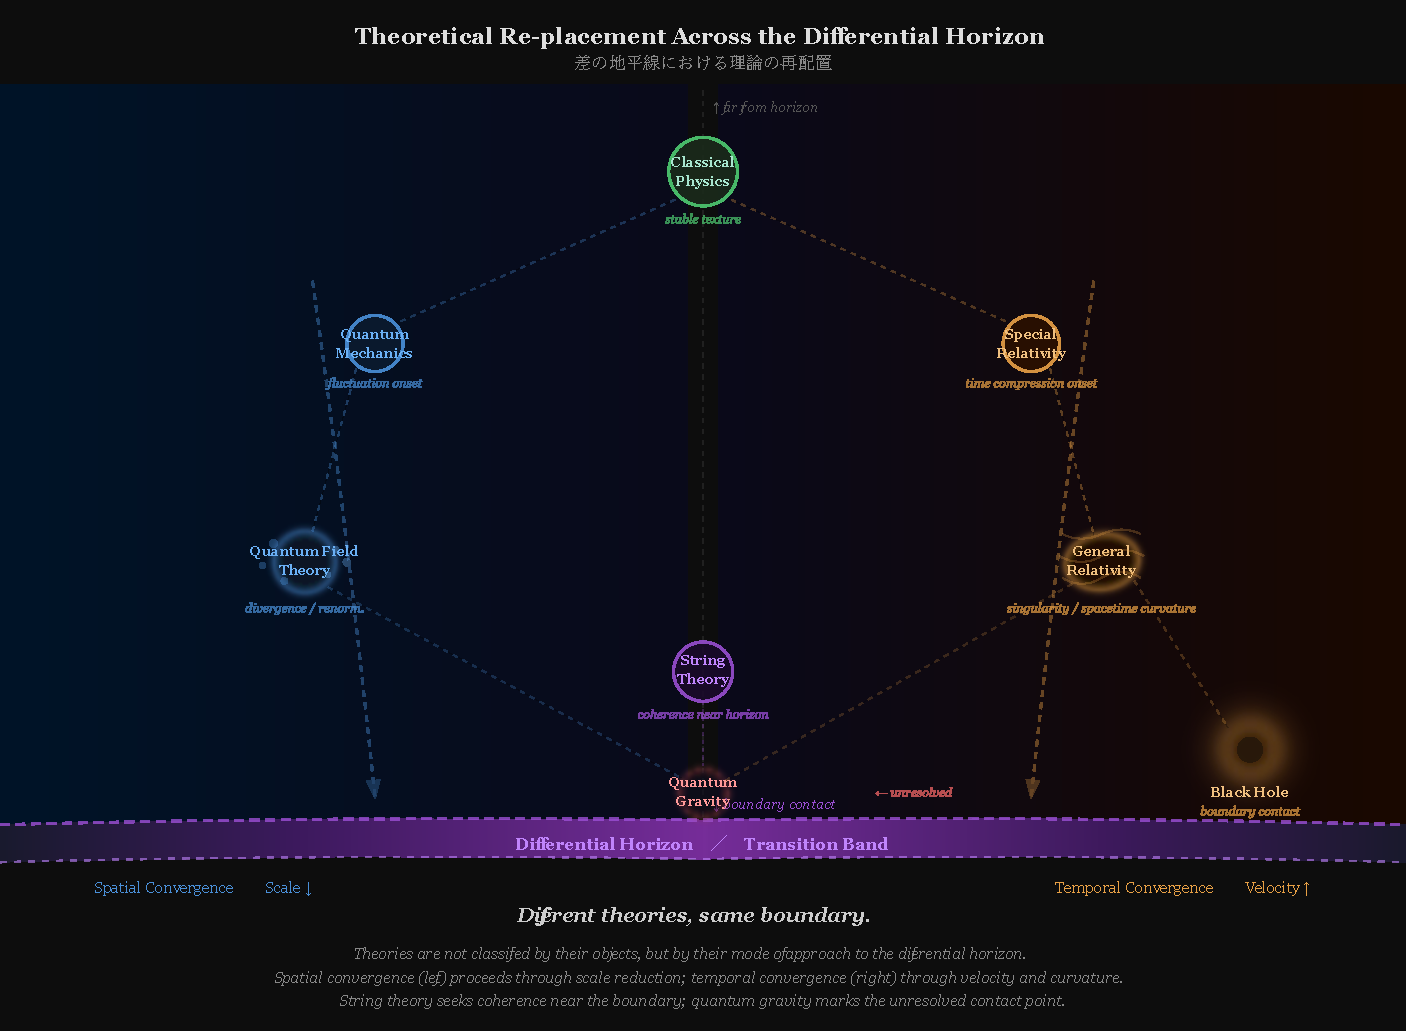
\includegraphics[width=\linewidth]{figures/figure3_theory_replacement.pdf}
  \caption{%
    Theoretical re-placement across local horizon-forms.
    Theories are organized not by their objects
    but by the observational windows they stabilize.
    Spatial convergence (left) encompasses quantum mechanics
    and quantum field theory.
    Temporal convergence (right) encompasses special
    and general relativity.
    Black holes occupy the \bcontact{} region.
    String theory seeks coherence where point-like description loses stability.
    Quantum gravity marks the unresolved contact point.
    The phrase ``same boundary'' in the schematic should be read
    structurally:
    different theories expose related local horizon-forms
    within their own descriptive windows.
    \textit{Different windows, related descriptive limits.}
  }
  \label{fig:theory_replacement}
\end{figure}

The next section shows how this unified view
gathers the major unsolved problems of modern physics
as local or hierarchical horizon-forms.
